\documentclass{beamer}

\usepackage[utf8]{inputenc}
\usepackage[ngerman]{babel}

\usepackage{array}
\usepackage{calc}
\usepackage{graphicx}
\usepackage{amssymb}
\usepackage{amsthm}
\usepackage{mathtools}
% \usepackage{xcolor}

\usepackage{algorithmicx}

\usepackage{algorithm}
\usepackage{algpseudocode}

\renewcommand{\algorithmicrequire}{\textbf{Input:}}
\renewcommand{\algorithmicensure}{\textbf{Output:}}


\usepackage{textpos}
\usepackage{color}
\usepackage{tikz}
\usetikzlibrary{shapes, arrows, positioning, decorations.pathmorphing}

\setbeamertemplate{bibliography item}[triangle]

\renewcommand{\atop}[2]{\genfrac{}{}{0pt}{2}{#1}{#2}}

\setbeamerfont{quote}{shape=\upshape,family=\rmfamily}

\newcommand{\mc}{\mathcal}
\newcommand{\mb}{\mathbf}
\newcommand{\N}{\mathbb{N}}
\newcommand{\Z}{\mathbb{Z}}
\newcommand{\Q}{\mathbb{Q}}
\newcommand{\R}{\mathbb{R}}
\newcommand{\Sy}{\mathcal{S}}
\newcommand{\tb}[1]{{\textcolor{blue}{#1}}}
\newcommand{\tred}[1]{{\textcolor{red}{#1}}}
\newcommand{\Nk}{\operatorname {Nk}}
\newcommand{\Nr}{\operatorname {Nr}}
\newcommand{\expand}{\texttt{KeyExpansion}}
\newcommand{\size}{\operatorname{size}}
\newcommand{\parf}{\operatorname{par}}
\newcommand{\GF}{\operatorname{GF}}
\newcommand{\ol}[1]{[#1]}

\theoremstyle{plain}
\newtheorem{thm}{Satz}[section]
\newtheorem{lem}[thm]{Lemma}
\newtheorem{prop}[thm]{Proposition}
\newtheorem{defn}[thm]{Definition}
\newtheorem{expl}[thm]{Beispiel}
\newtheorem{rem}[thm]{Bemerkung}
\newtheorem{cor}[thm]{Korollar}
\newtheorem{notn}[thm]{Notation}

\usetheme{Boadilla}
\setbeamertemplate{navigation symbols}{} %Leave out navigation symbols
 \setbeamertemplate{footline}
        {
      \leavevmode%
      \hbox{%
      \begin{beamercolorbox}[wd=.333333\paperwidth,ht=2.25ex,dp=1ex,center]{author in head/foot}%
        \usebeamerfont{author in head/foot}\insertshortauthor~~(\insertshortinstitute)
      \end{beamercolorbox}%
      \begin{beamercolorbox}[wd=.333333\paperwidth,ht=2.25ex,dp=1ex,center]{title in head/foot}%
        \usebeamerfont{title in head/foot}\insertshorttitle
      \end{beamercolorbox}%
      \begin{beamercolorbox}[wd=.333333\paperwidth,ht=2.25ex,dp=1ex,right]{date in head/foot}%
        \usebeamerfont{date in head/foot}\insertshortdate{}\hspace*{2em}

    %#turning the next line into a comment, erases the frame numbers
        %\insertframenumber{} / \inserttotalframenumber\hspace*{2ex} 

      \end{beamercolorbox}}%
      \vskip0pt%
    }
    
    
\title[AES]{Wie verschlüsselt Skype?}
\subtitle{Der Advanced Encryption Standard (AES)}
\author[Torchiani]{Carolin Torchiani}
\institute[Uni Koblenz]{\vspace{-0.5cm}\begin{center}
 
\includegraphics[width=27mm]{logo_uni-koblenz}
\end{center}
}

\date{Koblenz, 04.\ Mai 2015}


\begin{document}

\frame{\titlepage}

\addtobeamertemplate{frametitle}{~}{%
\begin{textblock*}{40mm}[0.75, 0.75](\textwidth, 0\textheight)

\includegraphics[width=27mm]{logo_uni-koblenz}
\end{textblock*}}

\tikzset{pblock/.style = {draw, rectangle split, rectangle split vertical,
                      rectangle split parts=2, very thick, fill=blue!20, rounded corners}}

                      
\begin{frame}{Advanced Encryption Standard (AES)}{Geschichte}
 
 \begin{block}{Advanced Encryption Standard}
 \begin{itemize}
  \item flächendeckend und weltweit genutzes Secret"=Key"=Kryptosystem
  \item komplexere Versionen in den USA für staatliche Dokumente mit höchster Geheimhaltungsstufe zugelassen
  \item mathematisches Konzept: Blockchiffre
 \end{itemize}
 \end{block}
 
 \begin{block}{Einsatz in der Praxis}
  \begin{itemize}
   \item Wireless LAN, z.\,B.~WPA2
   \item Netzwerkprotokolle, z.\,B.~SSH (Secure Shell)
   \item IP-Telefonie, z.\,B.~Skype
   \item Datenkomprimierung, z.\,B.~zip- und rar-Archive
  \end{itemize}
 \end{block}

\end{frame}

\begin{frame}{Advanced Encryption Standard (AES)}{\ }

\begin{block}{Geschichte}
 \begin{itemize}[<+->]
  \item Data Encryption Standard (DES)\\
  $\leadsto$ Vorgänger von AES\\
  $\leadsto$ 1977 vom US-amerikanischen National Institutue of Standards and Technology (NIST) eingeführt\\
  $\leadsto$ aufgrund schneller Computer Ende der 90er nicht mehr sicher
  \item 1997: NIST startet Wettbewerb, um einen Nachfolger für DES zu finden\\
  $\leadsto$ Gewinner: Joan Daemen und Vincent Rijmen\\
  $\leadsto$ Rijndael-Chiffre
  \item 2001: Standardisierung von AES\\
  $\leadsto$ weltweiter Einsatz
 \end{itemize}
\end{block}
\end{frame}

\begin{frame}{Advanced Encryption Standard (AES)}{\ }
\begin{block}{Sicherheit}
\begin{itemize}
 \item AES gilt bis heute als sicher
 \item 2011: erster erfolgreicher Angriff auf AES\\
 $\leadsto$ (nur) um Faktor $4$ schneller als vollständiges Durchsuchen des Schlüsselraums\\
 $\leadsto$ in der Praxis irrelevant
\end{itemize}
\end{block}
\end{frame}


\begin{frame}{AES: Blockchiffre}{\ }

\begin{block}{Grunddaten}
 \begin{itemize}
  \item \textbf{Alphabet}: endlicher Körper mit $256$ Elementen, der mit 
  \[\GF(2^8) = \GF(256)\]
  bezeichnet wird
  \item mehrere Versionen mit unterschiedlicher \textbf{Blocklänge} $\Nk = 16, 24, 32$ und unterschiedlich Anzahl der Runden
  \[\Nr = \begin{cases}
         10 & \text{ für } \Nk = 16,\\
         12 & \text{ für } \Nk = 24,\\
         14 & \text{ für } \Nk = 32\\
        \end{cases}\]
 \end{itemize}
 \end{block}
 \pause
 \begin{alertblock}{\ }
 \textbf{Im Vortrag}: Blocklänge $\Nk = 16$ und Rundenanzahl $\Nr = 10$
 \end{alertblock}
\end{frame}

\begin{frame}{Alphabet}{AES}
 
 \begin{block}{Warum $\GF(2^8)$ und nicht $\Z_p$ mit $p$ prim?}
  \begin{itemize}
   \item Computer arbeiten auf Bits und Bytes als kleinster Maßeinheit für Informationsgehalt
   \begin{enumerate}
    \item Bit: zwei Zustände, \emph{Ein} oder \emph{Aus}\\
    $\leadsto$ in der Mathematik $[0], [1] \in \Z_2$\\
    \item Bytes: bestehen aus $8$ Bits\\
    $\leadsto$ in der Mathematik Elemente von $\Z_2^8$\\
    $\leadsto$ z.\,B.~$(\ol 1, \ol 0, \ol 1, \ol 1, \ol 1, \ol 0, \ol 0, \ol 1) \in \Z_2^8$\\
    $\leadsto$ in der Regel kürzere Notation $10111001 \in \Z_2^8$
   \end{enumerate}
  \end{itemize}
 \end{block}
\end{frame}


\begin{frame}{Alphabet}{AES}
 
 \begin{block}{Warum $\GF(2^8)$ und nicht $\Z_p$ mit $p$ prim?}
  \begin{itemize}[<+->]
   \item Verschlüsselungsalgorithmen sollen schnell sein und wenig Speicher verbrauchen\\
   $\leadsto$ Nutzung der computereigenen Struktur mit $2^8$ Byte-Zuständen\\
   $\leadsto$ Alphabet mit $2^8 = 256$ Buchstaben
   \item Verschlüsselungsalgorithmen sollen komplexere Rechenoperationen auf dem Alphabet zulassen\\
   $\leadsto$ Alphabet, das ein Körper ist
  \end{itemize}
  \medskip
  \pause
  $\Rightarrow$  Köper $\GF(2^8)$ mit $256$ Elementen als Alphabet für AES
 \end{block}
\end{frame}

\begin{frame}{Zeichencodierung mittels UTF-8}{Noch ein Vorteil von 256 Buchstaben\dots}
 
 \begin{block}{Unicode und UTF-8}
  \begin{itemize}
   \item Unicode: langfristige Festlegung eines digitalen Codes für jedes Schriftzeichen
   \item UTF-8: am weitesten verbreitete Unicode-Codierung, Erweiterung von ASCII\\
   $\leadsto$ Anfang 2015 nutzen über $80\%$ der Webseiten UTF-8 zur Zeichencodierung
  \end{itemize}
 \end{block}
 \begin{center}
 \begin{tikzpicture}
  \node[draw, rounded corners] (Z) at (-3, 0) {Zeichen};
  \node[draw, rounded corners] (UC) at (0, 0) {Zahl};
  \node[draw, rounded corners, text width = 1.75cm] (UTF) at (3, 0) {Byte-Folge 1-4 Bytes};
  \draw[-latex] (Z) -- (UC);
  \draw[-latex] (UC) -- (UTF);
  
  \node[blue] (Z) at (-3, -1) {Text};
  \node[blue] (UC) at (0, -1) {Unicode};
  \node[blue] (UTF) at (3, -1) {UTF-8};
 \end{tikzpicture}
 \end{center}
\end{frame}

\begin{frame}{Zeichencodierung mittels UTF-8}{Noch ein Vorteil von 256 Buchstaben\dots}
 \begin{center}
 $
 \begin{rcases*}
  \texttt A \;\\
  \texttt E \;\\
  \texttt S \;
 \end{rcases*} 
 \underset{\text{UTF-8-codiert}}{\widehat{=}}
 \begin{cases}
  \;01000001 \\
  \;01000101 \quad \in \Z_2^8\\
  \;01010011
 \end{cases}
 $
 \bigskip
 
 \texttt{AES} $\underset{\text{UTF-8-codiert}}{\widehat{=}}$ $(01000001, 01000101, 01010011) \in (\Z_2^8)^3$
 \end{center} \pause
 
 \begin{block}{Zeichencodierung mittels UTF-8}
  Buchstaben vieler westlicher Sprachen brauchen häufig genau ein Byte Speicherplatz:
  \begin{center}
  \begin{tabular}{cl}
 & Buchstabe im menschenlesbaren Text \\
 $\widehat{=}$ & UTF-8-codiert genau ein Byte \\
 $\widehat{=}$ & einer von 256 Buchstaben im Alphabet von AES 
 \end{tabular}
  \end{center}
 \end{block}
\end{frame}

\begin{frame}{Zeichencodierung mittels UTF-8}{Noch ein Vorteil von 256 Buchstaben\dots}

 \begin{center}
  \begin{tikzpicture}
   \node[draw, rounded corners, fill=blue!10] (T1) at (-3, 4) {Text};
   \node[draw, rounded corners, fill=blue!10] (B1) at (-3, 2) {Byte-Folge};
   \node[draw, rounded corners, fill=blue!10] (B12) at (-3, 0) {Byte-Folge};
   \node[draw, rounded corners, fill=blue!10] (T2) at (3, 4) {Text};
   \node[draw, rounded corners, fill=blue!10] (B2) at (3, 2) {Byte-Folge};
   \node[draw, rounded corners, fill=blue!10] (B22) at (3, 0) {Byte-Folge};
   
   \node[blue] (S) at (-3, -1.5) {Sender};
   \node[blue] (E) at (3, -1.5) {Empfänger};
   
   \draw[-latex] (T1) -- node[left] {UTF-8} (B1);
   \draw[-latex] (B1) -- node[right] {AES} node[left] {Verschlüsselung} (B12);
   \draw[-latex] (B12) -- node[below] {Übertragung} (B22);
   \draw[-latex] (B22) -- node[right] {Entschlüsselung} node[left] {AES} (B2);
   \draw[-latex] (B2) -- node[right] {UTF-8} (T2);
  \end{tikzpicture}
 \end{center}

\end{frame}

\begin{frame}{Ein Körper mit 256 Elementen\dots}{$\GF(256) = \GF(2^8)$}
 
 \begin{block}{Satz}
  Seien $n \in \N$, $p \in \mathbb P$. Dann existiert ein Körper mit $p^n$ Elementen. Er ist bis auf Isomorphie eindeutig. Wir bezeichnen ihn mit $\GF(p^n)$. 
 \end{block}
\bigskip

 ``Bis auf Isomorphie eindeutig'':\\
 Wenn $K_1$ und $K_2$ zwei Körper mit $p^n$ Elementen sind, dann sind $K_1$ und $K_2$ isomorph.
 \pause
 \bigskip
 
 \tb{Insbesondere existiert ein Körper mit $256=2^8$ Elementen, nämlich $\GF(2^8)$.}
\end{frame}

\begin{frame}{Ein Körper mit 256 Elementen\dots}{$\GF(256) = \GF(2^8)$}        
Bezeichnung der Elemente von $\GF(2^8)$:
\begin{enumerate}
 \item Elemente von $\Z_2^8$, z.\,B.~$([0],[1],[0],[1],[0],[0],[1],[0]) \in \GF(2^8)$
 \item zweistellige Hexadezimalzahlen, z.\,B. $\texttt{d2}$\\
 (davon gibt es $16 \cdot 16 = 2^8$ Stück)
\end{enumerate}
\end{frame}

\begin{frame}{Hexadezimalsystem}{Stellenwertsystem zur Basis $16$}

Ziffern:\\
 \[\text{\texttt{0, 1, 2, 3, 4, 5, 6, 7, 8, 9, a, b, c, d, e, f}}\]
 \bigskip
 
 Beispiel:
 \begin{align*}
 \texttt{c}\; & \widehat{=} \; 12 \cdot 1 = 12\\
 \texttt{4c}\; & \widehat{=} \; 4 \cdot 16 + 12 \cdot 1 = 76\\
  \texttt{b4c}\; & \widehat{=} \; 11 \cdot 16^2 + 4 \cdot 16 + 12 \cdot 1 = 2892
 \end{align*}
 \pause
 \begin{alertblock}{Kürzere Darstellung von Elementen $(a_1, \dotsc, a_8) \in \Z_2^8 \; \widehat{=} \; \GF(2^8)$:}
 \begin{center}
$2$-stellige Zahl im Hexadezimalsystem
\end{center}
\end{alertblock}
 \end{frame}

 \begin{frame}{Hexadezimalsystem}{Stellenwertsystem zur Basis $16$}
\begin{block}{Beispiel}
\begin{center}
\begin{tikzpicture}
 \node (Z28) at (0, 6) {$(\ol 1, \ol 0, \ol 1, \ol 1, \ol 1, \ol 0, \ol 0, \ol 1) \in \Z_2^8$};
 \node (B) at (0, 5) {$10111001 \quad$ Binärsystem};
 \node (B1) at (-3, 4) {$1011 \quad$Binärsystem};
 \node (B2) at (3, 4) {$1001 \quad$ Binärsystem};
 \node (D1) at (-3, 3) {$11 \quad$ Dezimalsystem};
 \node (D2) at (3, 3) {$9 \quad$ Dezimalsystem};
 \node (H1) at (-3, 2) {$\texttt b \quad$ Hexadezimalsystem};
 \node (H2) at (3, 2) {$\texttt 9 \quad$ Hexadezimalsystem};
 \node (H) at (0, 1) {$\texttt {b9} \quad$ Hexadezimalsystem};
 \draw[latex-latex] (Z28) -- (B);
 \draw[latex-latex] (B) -- (B1);
 \draw[latex-latex] (B) -- (B2);
 \draw[latex-latex] (B1) -- (D1);
 \draw[latex-latex] (D1) -- (H1);
 \draw[latex-latex] (B2) -- (D2);
 \draw[latex-latex] (D2) -- (H2);
 \draw[latex-latex] (H2) -- (H);
 \draw[latex-latex] (H1) -- (H);
  \end{tikzpicture}
  \end{center}
\end{block}
\end{frame}


\begin{frame}{Addition auf $\GF(2^8)$}{AES}
\begin{itemize}
\item  Addition auf $\GF(2^8)$: Addition auf $\Z_2^8$
\bigskip

Beispiel:
\begin{center}
 $(\ol 1, \ol 0, \ol 1, \ol 1, \ol 1, \ol 0, \ol 0, \ol 1) + (\ol 1, \ol 1, \ol 0, \ol 1, \ol 0, \ol 1, \ol 0, \ol 1)$
 $= (\ol 0, \ol 1, \ol 1, \ol 0, \ol 1, \ol 1, \ol 0, \ol 0)$
\end{center}
\medskip
\item Multiplikation auf $\GF(2^8)$: wird nicht eingeführt
\end{itemize}
\end{frame}

\begin{frame}{Ein Körper mit 256 Elementen\dots}{AES}
 \begin{block}{Zusammenfassung}
  \begin{enumerate}
   \item $A = \GF(2^8)= \GF(256)$ als Alphabet der Blockchiffre AES
   \item Notation der Elemente von $\GF(2^8)$:
   \begin{enumerate}
   \item Elemente von $\Z_2^8$
   \item zweistellige Hexadezimalzahlen
  \end{enumerate}
  \item Blocklänge von AES: $n = 16$\\
  $\mc P = \mc C = \mc K = A^{16} = (\GF(2^8))^{16}$
  \end{enumerate}
 \end{block}
 \bigskip
 Beispiel:
 \begin{small}
 \[\texttt{32 43 f6 a8 88 5a 30 8d 31 31 98 a2 e0 37 07 34} \; \; \in \mc P = \GF(2^8)^{16}\]
 \end{small}
\end{frame}


\begin{frame}{Der AES-Algorithmus}{\ }
 Für einen Schlüssel $e \in \mc K = \GF(2^8)^{16}$, z.\,B.
 \begin{small}
 \[\texttt{3d c3 16 a3 28 ba a0 fd 3e 32 92 52 e0 b7 0b b4} \; \; \in \mc K = \GF(2^8)^{16},\]
 \end{small}
 beschreiben wir den Verschlüsselungsalgorithmus 
 \[E_e: \mc P = \GF(2^8)^{16} \rightarrow \mc C = \GF(2^8)^{16}.\]
 \bigskip
 \pause
 
 Erster Schritt:\\
 Erzeugung eines expandierten Schlüssel 
 \[\expand(e) = (e_1, \dots, e_{10}) \;\;\; \in  \mc K^{10} = (\GF(2^8)^{16})^{10}\]
\end{frame}

\begin{frame}{Expandierter Schlüssel}{Der AES-Algorithmus}
\begin{small}
 \begin{align*}
\texttt{29 ee cb 34 44 85 93 3a 5b d6 5c 47 9f 11 3a 70} & \\  
\texttt{32 43 f6 a8 88 5a 30 8d 31 31 98 a2 e0 37 07 34} & \\
\texttt{49 8f 52 43 1f e1 cb e2 bf 94 3c d0 30 f5 55 a0} & \\
\texttt{6e c2 63 7f 27 3b ee 7f f0 2f 74 ac 92 21 22 c6} & \\
\texttt{3b b9 73 ae c9 f1 7c 78 66 60 86 6e 85 9d 04 70} & \\
\texttt{ec 1a 11 21 0e 6b 86 1a a6 70 d5 04 a8 fc ff 5d} & \\
\texttt{0f de 2f aa 20 ce 47 5f da 09 42 22 b6 cc 2f ba} & \\
\texttt{db 7a 6a 30 7f e5 e2 07 52 94 24 4d 7c 19 62 37} & \\
\texttt{a8 fe c0 b7 58 16 8e 2c 4a de 6e 7c 8e eb 24 4a} & \\
\texttt{f0 34 ab 36 84 89 06 4e 29 3a 6b 0f 82 09 72 be} & \; \in \mc K^{10} = (\GF(2^8)^{16})^{10}
 \end{align*}
 \end{small}
\end{frame}

\begin{frame}{Der AES-Algorithmus}{\ }
 \begin{algorithmic}
  \Require Klartext $p \in \GF(2^8)^{16}$, Schlüssel $e \in \GF(2^8)^{16}$
  \Ensure Chiffretext $E_e(p) = c \in \GF(2^8)^{16}$
  \State $(e_1, \dots, e_{10}) \gets \expand(e)$
  \State $c \gets p + e$
  \For{$i = 1, \dots, 9$} 
  \State $c \gets$ \texttt{SubBytes}$(c)$
  \State $c \gets$ \texttt{ShiftRows}$(c)$
  \State $c \gets$ \texttt{MixColumns}$(c)$
  \State $c \gets c + e_i$
  \EndFor
  \State $c \gets $ \texttt{SubBytes}$(c)$
  \State $c \gets $ \texttt{ShiftRows}$(c)$
  \State $c \gets c + e_{10}$
  \State \Return $c$
 \end{algorithmic}
\end{frame}

\begin{frame}{\texttt{SubBytes}}{AES-Algorithmus}

\begin{block}{}$\texttt{SubBytes}: \GF(2^8)^{16} \rightarrow \GF(2^8)^{16}$ arbeitet \emph{buchstabenweise} durch Permutation des Alphabets $\GF(2^8)$.\end{block}

\begin{small}
 \[\sigma: \GF(2^8) \rightarrow \GF(2^8), \;\; b \mapsto A \tred{b^{-1}} + c\]
mit

\[A = \begin{pmatrix}
   \ol 1 & \ol 0 & \ol 0 & \ol 0 & \ol 1 & \ol 1 & \ol 1& \ol 1 \\
   \ol 1 & \ol 1 & \ol 0 & \ol 0 & \ol 0 & \ol 1 & \ol 1& \ol 1 \\
   \ol 1 & \ol 1 & \ol 1 & \ol 0 & \ol 0 & \ol 0 & \ol 1& \ol 1 \\
   \ol 1 & \ol 1 & \ol 1 & \ol 1 & \ol 0 & \ol 0 & \ol 0& \ol 1 \\
   \ol 1 & \ol 1 & \ol 1 & \ol 1 & \ol 1 & \ol 0 & \ol 0& \ol 0 \\
   \ol 0 & \ol 1 & \ol 1 & \ol 1 & \ol 1 & \ol 1 & \ol 0& \ol 0 \\
   \ol 0 & \ol 0 & \ol 1 & \ol 1 & \ol 1 & \ol 1 & \ol 1& \ol 0 \\
   \ol 0 & \ol 0 & \ol 0 & \ol 1 & \ol 1 & \ol 1 & \ol 1& \ol 1 \\
  \end{pmatrix} \in \Z_2^{8\times8} \text{ und } c = \begin{pmatrix}
							\ol 1 \\
							\ol 1 \\
							\ol 0 \\
							\ol 0 \\
							\ol 0 \\
							\ol 1 \\
							\ol 1 \\
							\ol 0
						      \end{pmatrix}.\]
\end{small}
\end{frame}

\begin{frame}{\texttt{SubBytes}}{AES-Algorithmus}
\begin{block}{}
 $\sigma: \GF(2^8) \rightarrow \GF(2^8)$ kann tabelliert werden. Z.\,B.:  $\sigma(\texttt{1d}) = \texttt{a4}$
\end{block}
\begin{center}
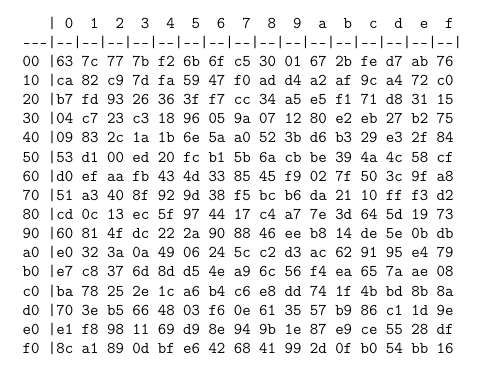
\includegraphics[scale=0.7]{subbytes}
\end{center}
\end{frame}


\begin{frame}{\texttt{SubBytes}}{AES-Algorithmus}
\begin{block}{}$\texttt{SubBytes}: \GF(2^8)^{16} \rightarrow \GF(2^8)^{16}$ arbeitet \emph{buchstabenweise} durch Permutation des Alphabets $\GF(2^8)$.\end{block}\medskip

\texttt{SubBytes} wendet die Permutation $\sigma$ buchstabenweise an:
\[\texttt{SubBytes}(p_1, \dots, p_{16}) = (\sigma(p_1), \dotsc, \sigma(p_{16}))\]
für alle $(p_1, \dots, p_{16}) \in \GF(2^8)^{16} = \mc P = \mc C$.
\bigskip

Zum Beispiel:
\begin{align*}
\texttt{SubBytes(}&\texttt{32 43 f6 a8 88 5a 30 8d 31 31 98 a2 e0 37 07 34)} \\
 =\;\;& \texttt{23 1a 42 c2 c4 be 04 5d c7 c7 46 3a e1 9a c5 18}.
 \end{align*}
 \end{frame}
 
 \begin{frame}{\texttt{ShiftRows}}{AES-Algorithmus}
 \begin{block}{}

 \texttt{ShiftRows} permutiert die Buchstaben von $p = (p_1, \dots, p_{16}) \in \GF(2^8)^{16}$:
   \begin{small}
\[\texttt{SubBytes}(p) = (p_1, p_6, p_{11}, p_{16}, p_5, p_{10}, p_{15}, p_4, p_9, p_{14}, p_3, p_8, p_{13}, p_2, p_7, p_{12})\]
\end{small}
\end{block}
\medskip

Zum Beispiel:
\begin{align*}
\texttt{ShiftRows(}&\texttt{23 1a 42 c2 c4 be 04 5d c7 c7 46 3a e1 9a c5 18)}\\
 =\;\;& \texttt{23 be 46 18 c4 c7 c5 c2 c7 9a 42 5d e1 1a 04 3a}\\
 \hline
 	           &\texttt{01 02 03 04 05 06 07 08 09 10 11 12 13 14 15 16} 
\end{align*}

 \end{frame}

 \begin{frame}{\texttt{MixColumns}}{AES-Algorithmus}
 \begin{block}{}
 \texttt{MixColumns} operiert auf Blöcken der Länge $4$, also auf $\GF(2^8)^4$. 
 \end{block}
\[S: \GF(2^8)^4 \rightarrow \GF(2^8)^4, \;\; \begin{pmatrix}
                                              p_1 \\
                                              p_2 \\
                                              p_3 \\
                                              p_4 
                                             \end{pmatrix}
 \mapsto \begin{pmatrix}
              \texttt{02} & \texttt{03} & \texttt{01} & \texttt{01} \\
              \texttt{01} & \texttt{02} & \texttt{03} & \texttt{01} \\
              \texttt{01} & \texttt{01} & \texttt{02} & \texttt{03} \\
              \texttt{03} & \texttt{01} & \texttt{01} & \texttt{02}
             \end{pmatrix} 
             \begin{pmatrix}
              p_1 \\
              p_2 \\
              p_3 \\
              p_4
             \end{pmatrix}.
\]

\begin{center}
\begin{footnotesize}
Einträge der Matrix: Hexadezimalzahlen, die für Elemente von $\GF(2^8)$ stehen  
\end{footnotesize}
\end{center}

\begin{block}{}
Die Transformation \texttt{MixColumns} wendet die $\GF(2^8)$-lineare Abbildung $S$ blockweise auf $(p_1, \dots, p_{16}) \in \GF(2^8)^{16}$ an:
\medskip

\begin{small}
$\texttt{MixColumns}(p)$

$= \left(S(p_1, p_2, p_3, p_4), S(p_5, p_6, p_7, p_8), S(p_9, p_{10}, p_{11}, p_{12}), S(p_{13}, p_{14}, p_{15}, p_{16})\right)$
\end{small}
\end{block}
 \end{frame}
 
 
\begin{frame}{Zusammenfassung}{Der AES-Algorithmus}
 \begin{algorithmic}
  \Require Klartext $p \in \GF(2^8)^{16}$, Schlüssel $e \in \GF(2^8)^{16}$
  \Ensure Chiffretext $c \in \GF(2^8)^{16}$
  \State $(e_1, \dots, e_{10}) \gets \expand(e)$
  \State $c \gets p + e$
  \For{$i = 1, \dots, 9$} 
  \State $c \gets$ \texttt{SubBytes}$(c)$
  \State $c \gets$ \texttt{ShiftRows}$(c)$
  \State $c \gets$ \texttt{MixColumns}$(c)$
  \State $c \gets c + e_i$
  \EndFor
  \State $c \gets $ \texttt{SubBytes}$(c)$
  \State $c \gets $ \texttt{ShiftRows}$(c)$
  \State $c \gets c + e_{10}$
  \State \Return $c$
 \end{algorithmic}
\end{frame}

\end{document}



